\documentclass[12pt, oneside]{book}
\usepackage[a4paper,top=2.5cm,bottom=2.5cm,left=3.5cm,right=2cm]{geometry}
\usepackage[utf8]{inputenc}
\usepackage[T1]{fontenc}
\usepackage{graphicx}
\usepackage{url}
%\usepackage[slovak]{babel} % vypnite pre prace v anglictine
\linespread{1.25} % hodnota 1.25 by mala zodpovedat 1.5 riadkovaniu

% my includes
\usepackage{color}
\usepackage{tocloft}
\usepackage{comment}
\usepackage{moreverb}
\usepackage{amsmath}
\usepackage{amsfonts}
\usepackage{amssymb}

\usepackage{enumitem}
\newlist{Algo}{enumerate}{1}
\setlist[Algo]{label=\textbf{Step \arabic*:}}

\usepackage[sort&compress]{natbib}
\bibpunct{[}{]}{,}{n}{,}{,}

\usepackage{listings}
\lstset{
language=Java,
basicstyle=\scriptsize\ttfamily,
%numbers=left,
%numberstyle=\tiny\color{lightblue},
%stepnumber=1,
%numbersep=15pt,
showspaces=false,
showstringspaces=false,
tabsize=4,
breaklines=true,
keywordstyle=\color{darkblue}\bfseries,
ndkeywordstyle=\color{gray}\bfseries,
commentstyle=\color{gray}\em,
stringstyle=\color{red},
frame=single % for frames around the code blocks
}
\definecolor{linkcolor}{rgb}{0, 0.4, 0.7}
\definecolor{blue}{rgb}{0,0.4,0.7}
\definecolor{darkblue}{rgb}{0,0.3,0.6}
\definecolor{gray}{rgb}{0.4,0.4,0.4}
\definecolor{lightgray}{rgb}{0.7,0.7,0.7}
\definecolor{red}{rgb}{1,0.05,0.05}
\definecolor{darkred}{rgb}{0.8,0,0}
\definecolor{lightblue}{rgb}{0.2,0.6,0.9}
\definecolor{black}{rgb}{0,0,0}


% -------------------
% --- Definicia zakladnych pojmov
% --- Vyplnte podla vasho zadania
% -------------------
\def\mfrok{2016}
%\def\mfnazov{Názov vašej bakalárskej práce}
%\def\mftyp{Bakalárska práca}
%\def\mfautor{Meno Priezvisko, príp. tituly}
%\def\mfskolitel{tit. Meno Priezvisko, tit. }
\def\mfnazov{Image-based steganography using a~mobile~phone}
\def\mftyp{Bachelor's thesis}
\def\mfautor{Askar Gafurov}
\def\mfskolitel{RNDr. Michal Forišek, PhD.}

%ak mate konzultanta, odkomentujte aj jeho meno na titulnom liste
\def\mfkonzultant{tit. Meno Priezvisko, tit. }  

\def\mfmiesto{Bratislava, \mfrok}

%aj cislo odboru je povinne a je podla studijneho odboru autora prace
%\def\mfodbor{2508 Informatika} 
%\def\program{ Informatika }
%\def\mfpracovisko{ Katedra informatiky }
\def\mfodbor{2508 Computer Science} 
\def\program{ Computer Science }
\def\mfpracovisko{ Department of Computer Science }

%% my macros
\def\TODO{\textbf{\textcolor{red}{TODO }}}
\def\app#1#2#3{\emph{#1} (by~#2) \url{#3}}
\def\ack#1#2{#1,\\#2\smallskip}
\begin{document}     

% -------------------
% --- Obalka ------
% -------------------
\thispagestyle{empty}

\begin{center}
\sc\large
%Univerzita Komenského v Bratislave\\
%Fakulta matematiky, fyziky a informatiky
Comenius University in Bratislava\\
Faculty of Mathematics, Physics and Informatics


\vfill

{\LARGE\mfnazov}\\
\mftyp
\end{center}

\vfill

{\sc\large 
\noindent \mfrok\\
\mfautor
}

\eject % EOP i
% --- koniec obalky ----

% -------------------
% --- Titulný list
% -------------------

\thispagestyle{empty}
\noindent

\begin{center}
\sc  
\large
%Univerzita Komenského v Bratislave\\
%Fakulta matematiky, fyziky a informatiky
Comenius University in Bratislava\\
Faculty of Mathematics, Physics and Informatics

\vfill

{\LARGE\mfnazov}\\
\mftyp
\end{center}

\vfill

\noindent
\begin{tabular}{ll}
%Študijný program: & \program \\
%Študijný odbor: & \mfodbor \\
%Školiace pracovisko: & \mfpracovisko \\
%Školiteľ: & \mfskolitel \\
Study program: & \program \\
Branch of studies: & \mfodbor \\
%Školiace pracovisko: & \mfpracovisko \\
Supervisor: & \mfskolitel \\
% Konzultant: & \mfkonzultant \\
\end{tabular}

\vfill


\noindent \mfmiesto\\
\mfautor

\eject % EOP i


% --- Koniec titulnej strany


% -------------------
% --- Zadanie z AIS
% -------------------
% v tlačenej verzii s podpismi zainteresovaných osôb.
% v elektronickej verzii sa zverejňuje zadanie bez podpisov

\newpage 
\thispagestyle{empty}
\hspace{-2cm}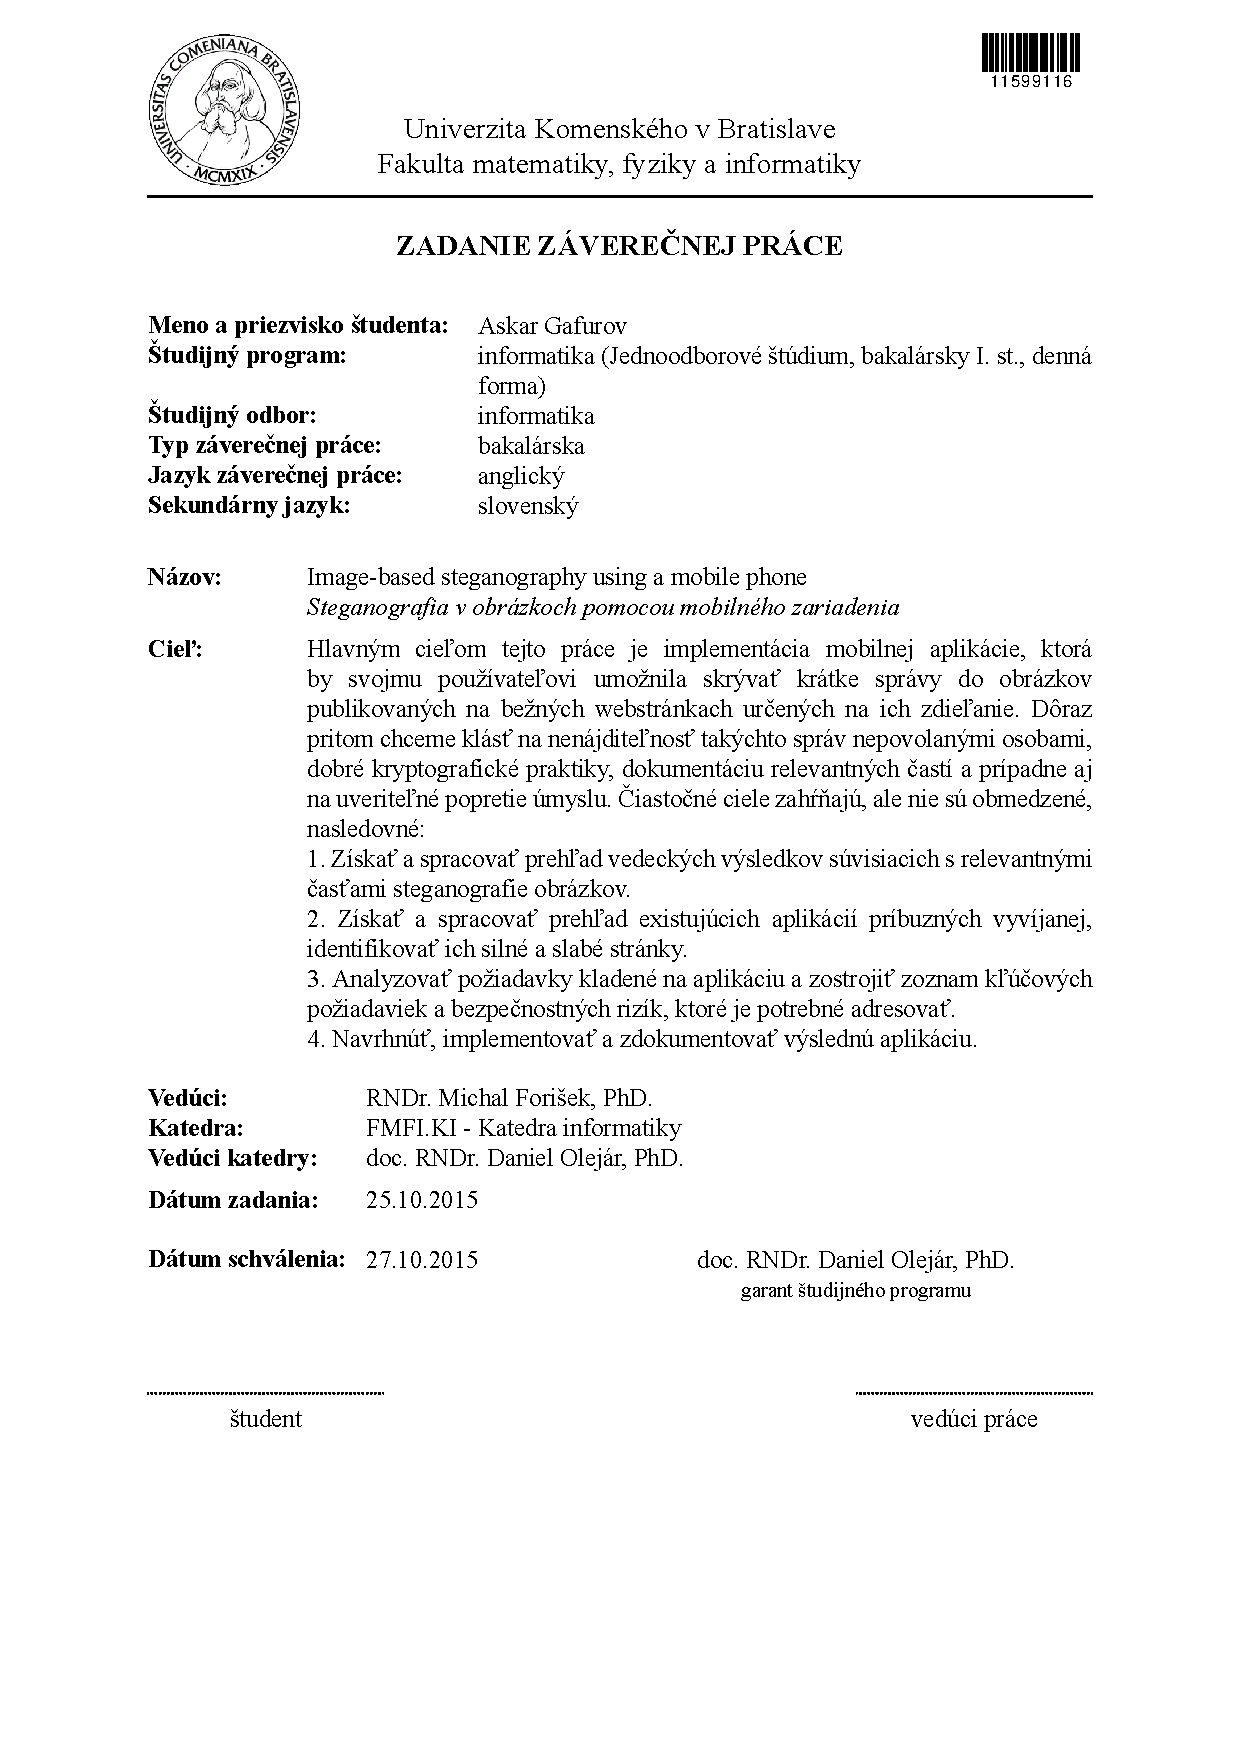
\includegraphics[width=1.1\textwidth]{images/zadanie_sk}

\newpage 
\thispagestyle{empty}
\hspace{-2cm}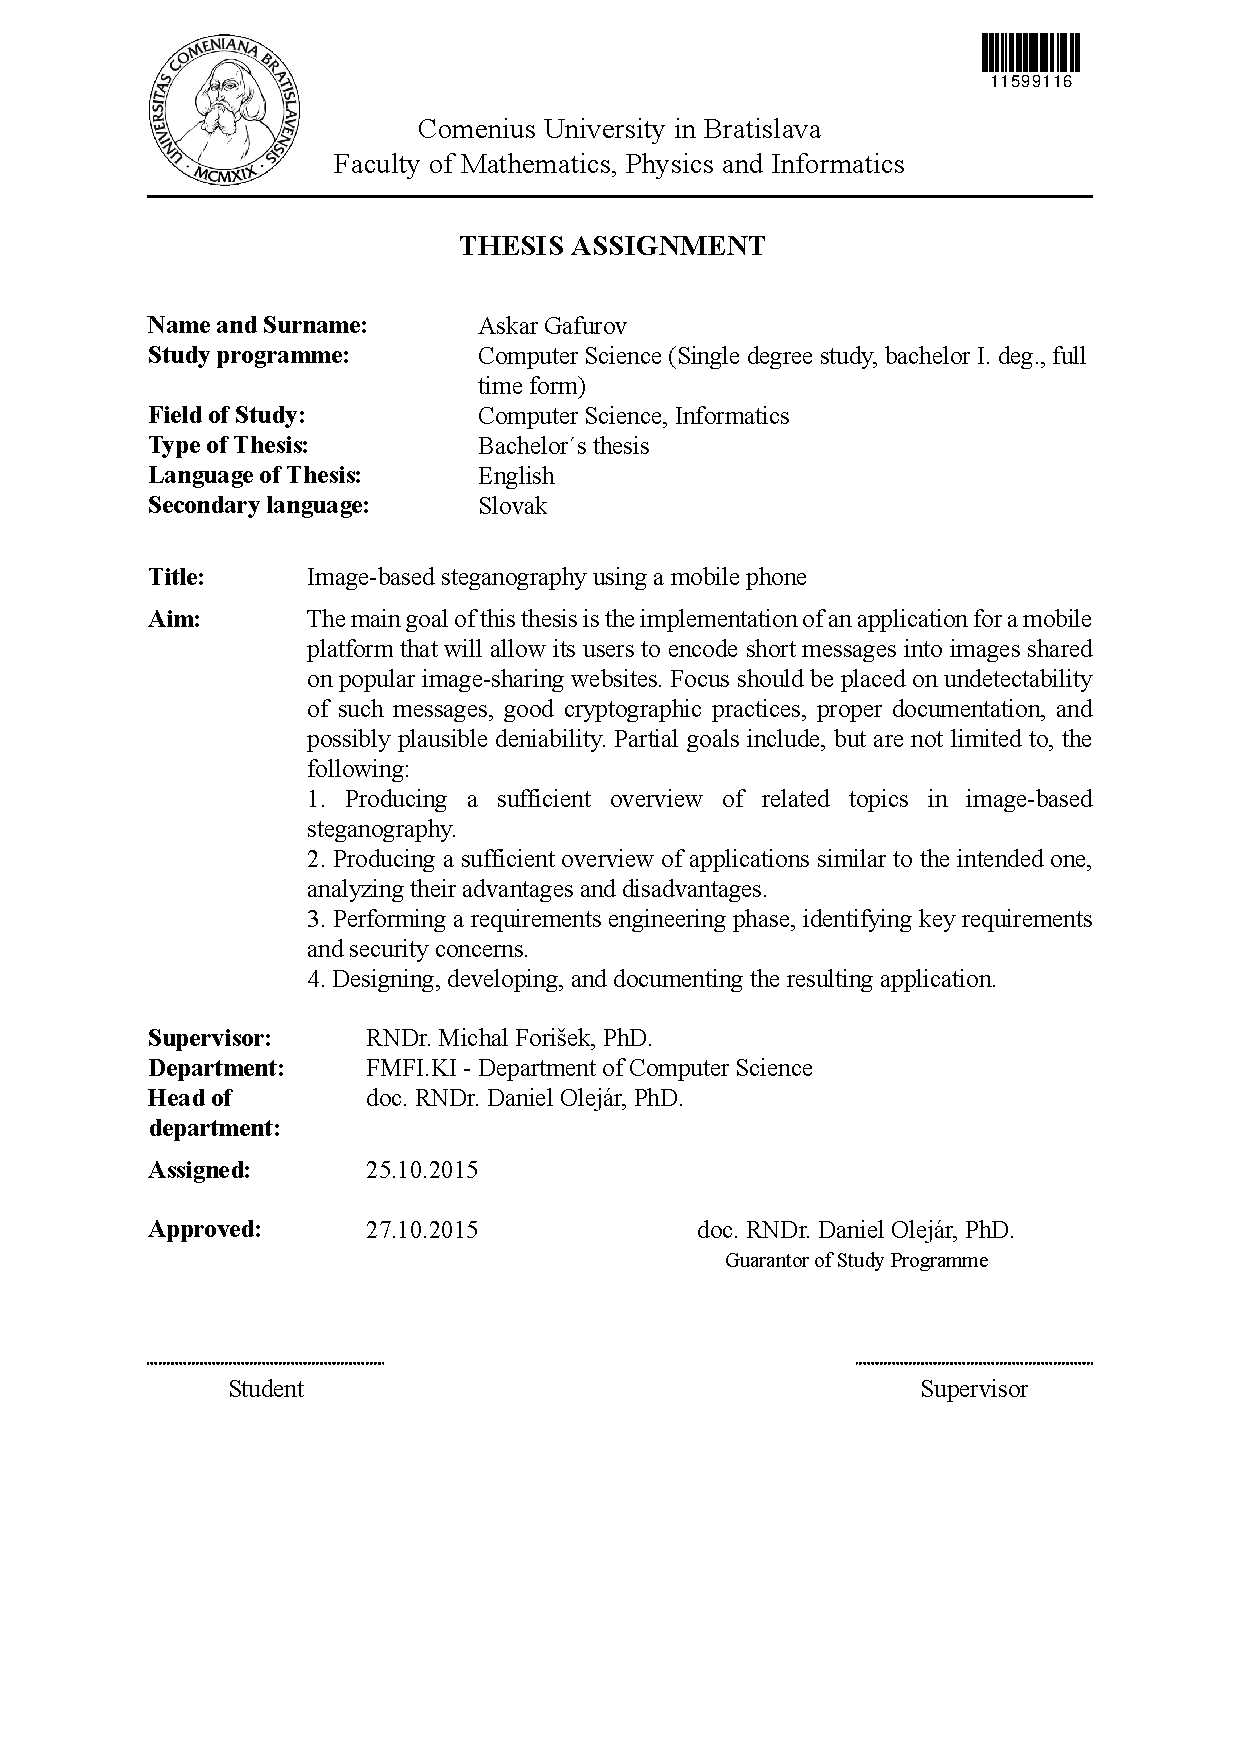
\includegraphics[width=1.1\textwidth]{images/zadanie_en}


% --- Koniec zadania

\frontmatter

% -------------------
%   Poďakovanie - nepovinné
% -------------------
\setcounter{page}{3}
\newpage 
~

\vfill
%{\bf Poďakovanie:}
{\bf Acknowledgements:} 

I'd like to thank:

\ack{my family}{for constantly pushing me out of my comfort zone,}

\ack{my primary school teachers Nayla Galiyeva and Nina Medvedeva}{for inviting me into 
a beautiful world of Mathematics,}

\ack{German Nurlygayanov}{for inviting me into a beautiful world of programming,}

\ack{Konstantin Ermolin, Alexandr Dulyasov and Emil Vakhitov}{for teaching me the art of friendship,}

\ack{doc. Dmitriy Kuznetzov}{for teaching me how to lose and how to win,}

\ack{my secondary school teachers RNDr. Zuzana Frková, PhDr. Daniela Veselovská, PaedDr. Pavol Danko and RNDr. Martin Kollár, PhD.}
{for helping me to acclimatize in Slovakia,}

\ack{Trojsten}{for giving me new friends and supporting my interest in Math and Computer~Science,}

\ack{Michal Smolík, Jaroslav Petrucha, Vladimír Macko, Jakub Šafin and Kamila Součková}{for being
my rivals and friends,}

\ack{doc. RNDr. Radoslav Harman, PhD.}{for inviting me into a beautiful world of Statistics,}

\ack{RNDr. Michal Forišek, PhD.}{for ignoring my e-mails and thus contributing to my independence,}

\ack{Adam Dej}{for providing his deep knowledge of software development,}

\ack{Mgr. Mária Božová and Nina Hronkovičová}{for supporting me in times of despair,}

and many others, without whom this would not have been possible.

\begin{comment}
I'd like to thank my supervisor RNDr. Michal Forišek, PhD. 
for ignoring my e-mails and thus contributing to my independence
and character development.
\end{comment}


\vfill

% --- Koniec poďakovania

% -------------------
%   Abstrakt - Slovensky
% -------------------
\newpage 
\section*{Abstrakt}

\begin{comment}
Slovenský abstrakt v rozsahu 100-500 slov, jeden odstavec. Abstrakt
stručne sumarizuje výsledky práce. Mal by byť pochopiteľný pre bežného
informatika. Nemal by teda využívať skratky, termíny alebo označenie
zavedené v práci, okrem tých, ktoré sú všeobecne známe.
\end{comment}

V tejto práci sme sa venovali digitálnej steganografii (ukrývaniu správ) pomocou obrázkov 
a konkretne steganografickým aplikáciám pre smartfóny s operačným systémom Android. 
Popisali sme momentálny stav poznania v tejto oblasti. 
Potom sme rozanalyzovali súčasné aplikácie
a popisali sme ich chyby. Na základe týchto vysledkov sme navrhli 
požiadavky, ktoré by mali takéto aplikácie spĺňať na to, aby boli efektívne. Následne
sme vyvinuli aplikáciu, ktorá danú špecifikáciu spĺňa. 
Pri tom sme priniesli implementáciu nového steganografického algoritmu a kostru
pre použitie nových steganografických metód.

\paragraph*{Kľúčové slová:} steganografia, Android, open-source, JPEG, komplementárne vkládanie 
% --- Koniec Abstrakt - Slovensky


% -------------------
% --- Abstrakt - Anglicky 
% -------------------
\newpage 
\section*{Abstract}

In this paper we've addressed digital image-based steganography (message hiding) and 
specifically steganographic applications for Android smartphones. We've overviewed modern
steganographic and steganalytic methods and mistakes of currently available steganographic
applications. With that in mind, we've deduced requirements to an application, that would
help it to avoid these mistakes. Then we developed such application. As byproduct, we've
brought free open-source Java implementation of complementary embedding algorithm, which
is superior to currently widely used F5 algotithm.


\paragraph*{Keywords:} steganography, Android, open-source, JPEG, complementary embedding

% --- Koniec Abstrakt - Anglicky

% -------------------
% --- Obsah
% -------------------

\newpage 

\tableofcontents

% ---  Koniec Obsahu

% -------------------
% --- Zoznamy tabuliek, obrázkov - nepovinne
% -------------------

\newpage 

\listoffigures

% ---  Koniec Zoznamov

\mainmatter

\input introduction.tex

%\part{EXISTED KNOWLEDGE}

\input steganography.tex

%\part{OUR WORK}

\input goals.tex

\input theory.tex

\input implementation.tex

\input summary.tex

% -------------------
% --- Bibliografia
% -------------------


\newpage	

\backmatter

\thispagestyle{empty}
\nocite{*}
\clearpage

%\bibliographystyle{plain}
\bibliographystyle{unsrt}
\bibliography{literatura} 


% -------------------
%--- Prilohy---
% -------------------

%Nepovinná časť prílohy obsahuje materiály, ktoré neboli zaradené priamo  do textu. Každá príloha sa začína na novej strane.
%Zoznam príloh je súčasťou obsahu.
%
%\addcontentsline{toc}{chapter}{Appendix A}
%\input manual.tex
%
%\addcontentsline{toc}{chapter}{Appendix B}
%\input AppendixB.tex

\end{document}
